\chapter{Diseño de la solución}
\textit{El desarrollo de una aplicación multiplataforma es una opción cada vez más a tener en 
cuenta dentro del ámbito del desarrollo móvil~\cite{10.1145/3241739}. La mayor parte de desarrollos
se van a querer destinar a las principales plataformas móviles, 
con el fin de llegar al máximo número de usuarios posibles.
}

\section{Tecnología empleada}
Como se había decidido en el segundo capítulo, la realización de este \textit{MVP} irá dirigido para las
plataformas móviles: \textit{Android} e \textit{iOS}. El desarrollo de una aplicación \textit{nativa} para 
cada sistema, evidentemente, no sería factible, ya que implicaría el doble de esfuerzo en la codificación,
testing y mantenimiento del producto~\cite{10.1145/2480362.2480464}.

Por ello, es necesario el uso de un \textit{framework} de ámbito multiplataforma que nos proporcione un
soporte para ambas plataformas. En este caso, se ha optado por la prometedora herramienta de desarrollo
impulsada por \textit{Google}: \textit{Flutter}.

\subsection{Flutter y Dart}
\textit{Flutter} junto a su lenguaje de programación principal, \textit{Dart}, buscan 
aproximar al usuario la apariencia y rendimiento 
propio al de un desarrollo \textit{nativo}, aprovechando todas las ventajas que proporciona 
un \textit{framework multiplataforma}~\cite{7934674}.

\begin{figure}[H]
    \centering
    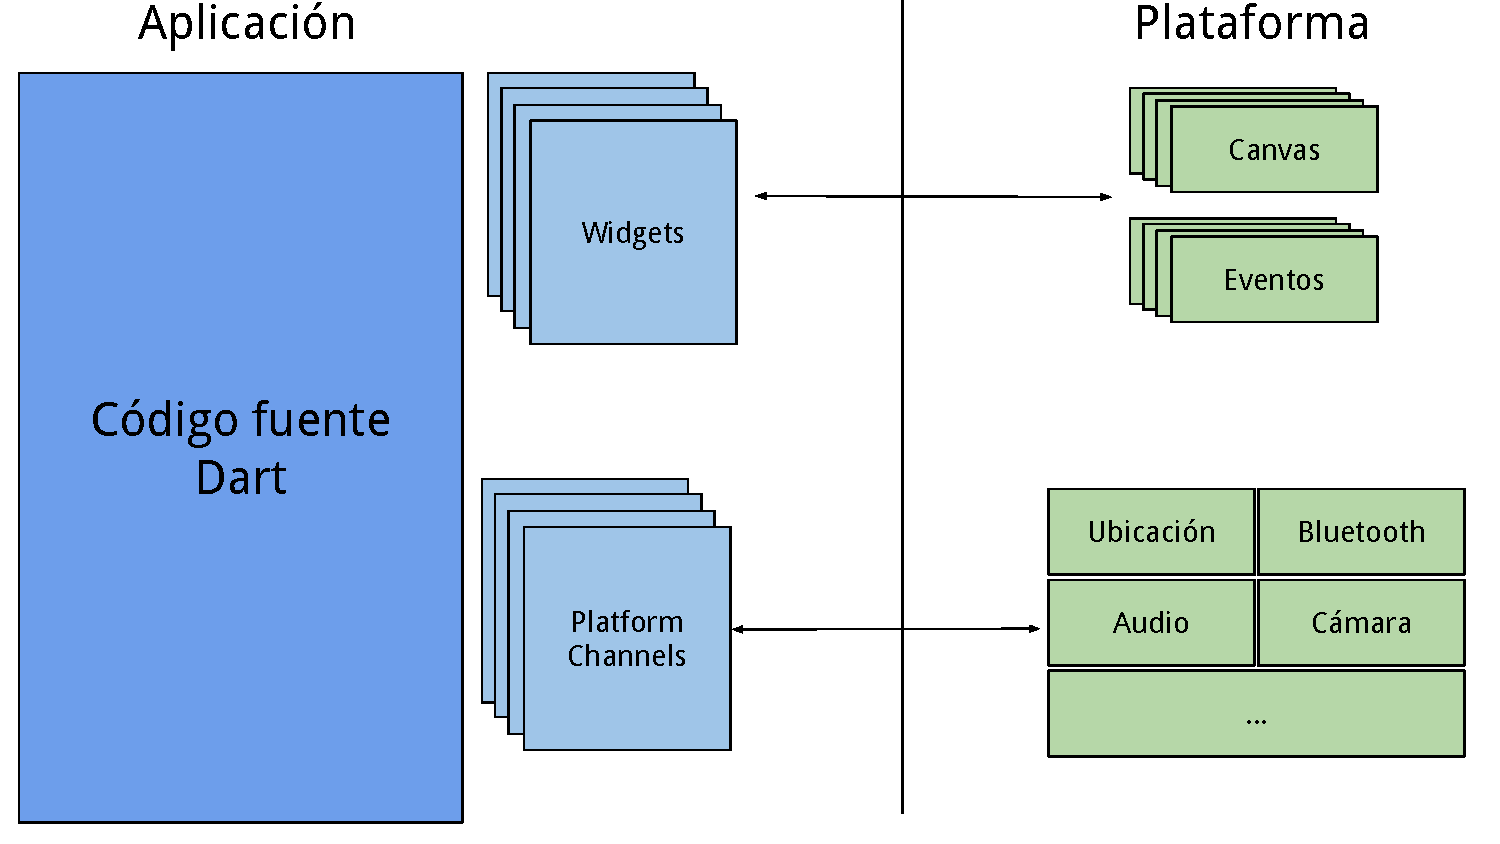
\includegraphics[scale=0.45]{images/flutter1.pdf}
    \caption{Diagrama de renderización de \textit{Flutter}\cite{leler2019s}}
    \label{fig:flutter1}
  \end{figure}

Esta relación \textit{apariencia/rendimiento}, la consigue \textit{Flutter} de forma exitosa
\textit{renderizando} directamente sus componentes, 
\textit{widgets}, en un \textit{canvas}, permitiendo visualizar el mismo componente en las diferentes plataformas.

Del mismo modo, realiza la conversión directa de servicios propios, \textit{Platform Channels}, en librerías nativas que
interactúan con las funcionalidades propias del dispositivo~\cite{leler2019s}, 
tal y como se puede visualizar en la Figura \ref{fig:flutter1}.

Esta en una de las razones principales por las que se ha elegido el uso de esta herramienta, frente a otros 
\textit{frameworks} de desarrollo móvil como: 

\begin{itemize}
    \item[$\bullet$] \textit{Frameworks de desarrollo móvil basados en Javascript} como: \textit{React Native} y 
    \textit{Vue Native}, que necesitan de una
    capa adicional para realizar la conversión a \textit{componentes nativos}, pudiendo afectar al rendimiento.
    \item[$\bullet$] Los \textit{frameworks embebidos} como
    \textit{Ionic} que emplea un \textit{WebView} para mostrar los componentes, dando la sensación de que no estás ejecutando
    una aplicación móvil, sino un sitio web embebido.
 \end{itemize}

 \subsection{Firebase}
 Para todas las funcionalidades relacionadas con servicios \textit{en nube}, vistos en la fase de Análisis,
 se empleará la plataforma de desarrollo backend impulsada y recomendada por \textit{Google}: \textit{Firebase}.

Gracias a que \textit{Firebase} presenta una base de datos del tipo \textit{real-time}, se permitirá 
la sincronización de los datos durante la ejecución del
aplicativo~\cite{khawas2018application}. Esta característica resulta ideal, ya que
\textit{Flutter}, al tratarse de un \textit{framework "declarativo"} no requiere de eventos para
sincronizar los datos, permitiendo al usuario visualizar los datos, en todo momento, sincronizados en pantalla,
sin necesidad de que el usuario realice un \textit{input de refrescar}.

Resulta muy potente esta propiedad, ya que la han querido adoptar los frameworks de desarrollo móvil nativo principales,
con aproximaciones como: \textit{SwiftUI} para aplicaciones \textit{iOS} y \textit{Jetpack Compose} para soluciones \textit{Android}.

Además, esta, al pertenecer al tipo de las \textit{no relacionales}, presenta ciertos beneficios frente a 
las \textit{relacionales},
a tener en cuenta en la definición de los modelos, tales como flexibilidad, seguridad y rendimiento.

La funcionalidades \textit{in-cloud} del \textit{back-end} de la aplicación final 
quedarán cubiertas por los apartados mostrados en la Tabla \ref{fig:tableFirebase}

\begin{table}[H]
    \centering
    \caption{Funcionalidades \textit{en nube} cubiertas por \textit{Firebase}}
      \begin{tabular}{ | c | c |}
        \hline
        \thead{Funcionalidad} & \thead{Tecnología} \\
        \hline
        \makecell{Autentificación} &  \makecell{\textbf{Firebase Authentication}, permite al usuario el acceso a las funciones de \\ la plataforma
        mediante inicio sesión tradicional \\ (cuenta de correo y contraseña)  o por RRSS.} \\
        \hline
        \makecell{Base de datos} &   \makecell{\textbf{Firebase Firestore}, permite al usuario interactuar mediante \\ funciones CRUD 
        la base de datos del sistema.} \\
        \hline
        \makecell{Analíticas} &  \makecell{\textbf{Firebase Analytics}, monitoriza la experiencia de usuario y extrae\\ estadísticas de cara 
        al lanzamiento de futuras versiones tales como:\\ porcentaje de usuarios libre de errores y número de usuarios activos.} \\
        \hline
      \end{tabular}
      \label{fig:tableFirebase}
  \end{table}

El diagrama de flujo del aplicativo con los servicios que ofrece la plataforma \textit{Firebase} puede verse
representado por el diagrama de la Figura\ref{fig:backdiagram1}

\begin{figure}[H]
  \centering
  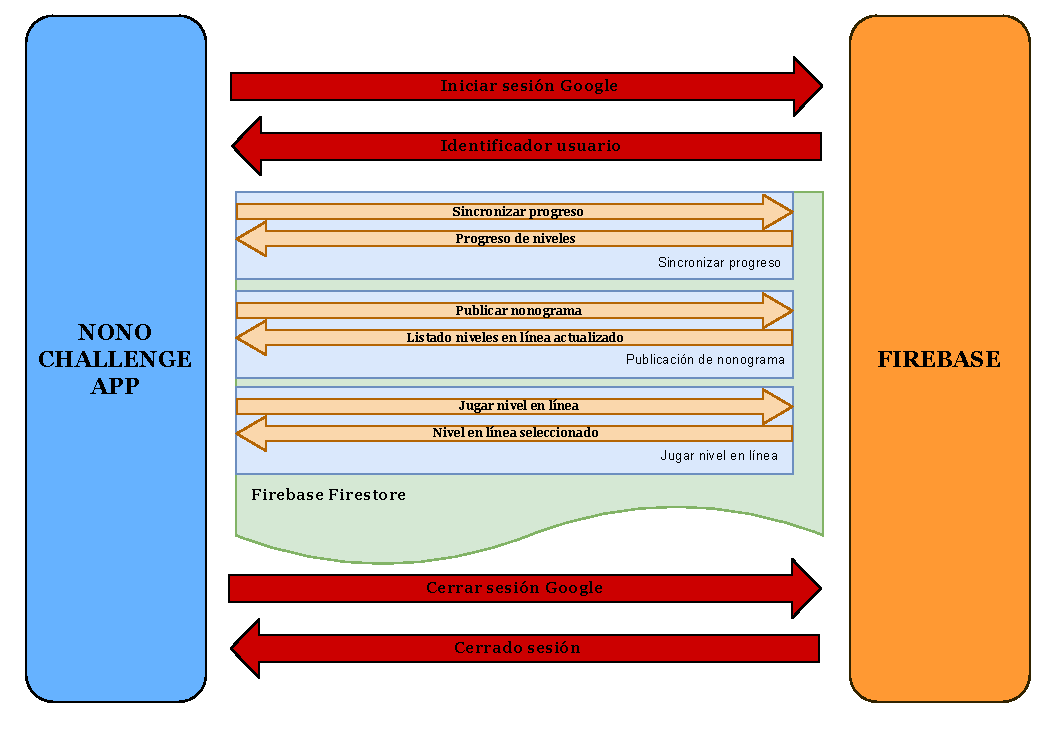
\includegraphics[scale=0.8]{images/back_diagram.pdf}
  \caption{Diagrama de flujo con \textit{Firebase}}
  \label{fig:backdiagram1}
\end{figure}

La gestión del progreso y publicación/resolución de niveles en línea se realizará mediante la función de \textit{Cloud Firestore},
para ello todas las transacciones se realizarán a través del identificador único de usuario.

\begin{figure}[H]
  \centering
  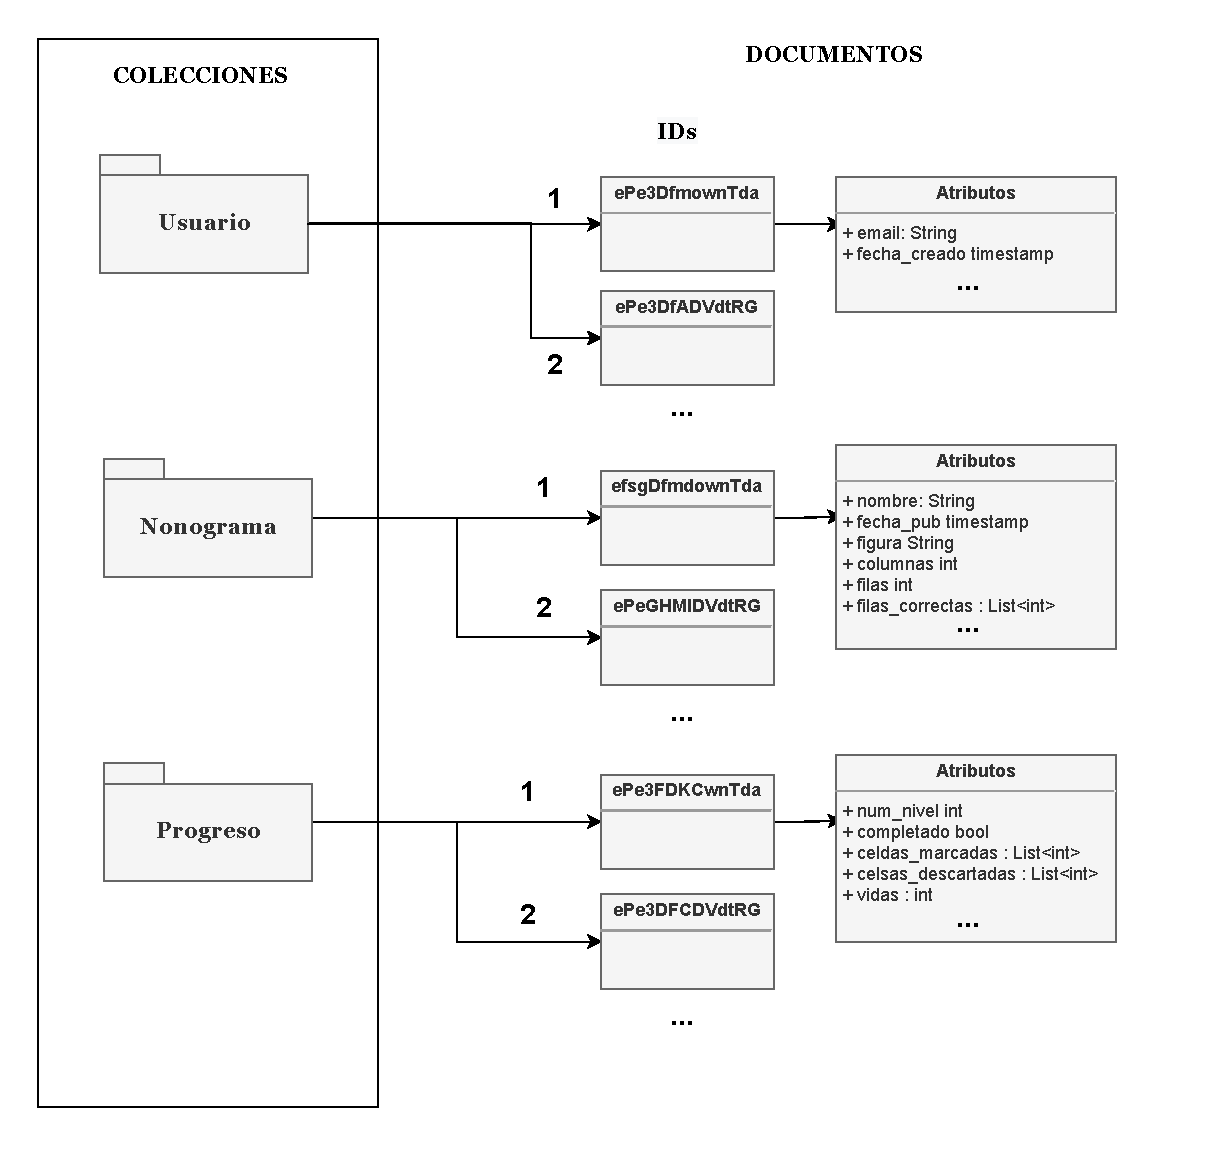
\includegraphics[scale=0.55]{images/firestore.pdf}
  \caption{Diagrama de estructura de datos de \textit{Firestore}}
  \label{fig:firestore1}
\end{figure}

En cuanto a la estructuración de los datos, al tratarse de una base de datos no relacional,
de tipo \textit{NoSql}, se tratarán los datos en forma de \textit{documentos}, cada uno con una clave identificativa única y una
serie de atributos. Estos documentos se almacerán según su tipo en contenedores llamados \textit{colecciones}:
\textit{usuarios, nonogramas y progresos}, en el caso de este aplicativo.

Este modelo de datos, a diferencia de los relacionales, puede ser totalmente flexible y definido por el aplicativo, no obstante,
para asegurar una mayor consistencia se ha definido desde el portal web de \textit{Firestore}, Figura \ref{fig:firestore1}.

  \subsection{Visual Studio Code}
Como \textit{IDE} de desarrollo se empleará la herramienta \textit{Visual Studio Code}, desarrollado por
\textit{Microsoft}, frente a otros entornos como: \textit{XCode} y \textit{Android Studio}, ya que este dispone
de una gran cantidad de \textit{extensiones o plugins}, que facilitan notablemente el proceso de \textit{codificación},
además de estar mejor optimizado para labores de \textit{compilación y depuración.}

\subsection{GitHub}
Se empleará \textit{GitHub} para el \textit{control de versiones}, siguiendo la metodología propias de 
\textit{GitFlow}, en el que tendremos, como se puede visualizar en la Figura~\ref{fig:gitflow1}:
i) una rama \textit{master} para versiones finales del aplicativo,
ii) una rama \textit{develop} en la que aunar las funcionalidades desarrolladas y iii) las ramas
\textit{feature} que se crearán por cada funcionalidad a desarrollar, dividida por todas las capas propuestas
por la filosofía \textit{Clean Architectute}, junto a sus \textit{suites de tests}.

\begin{figure}[H]
    \centering
    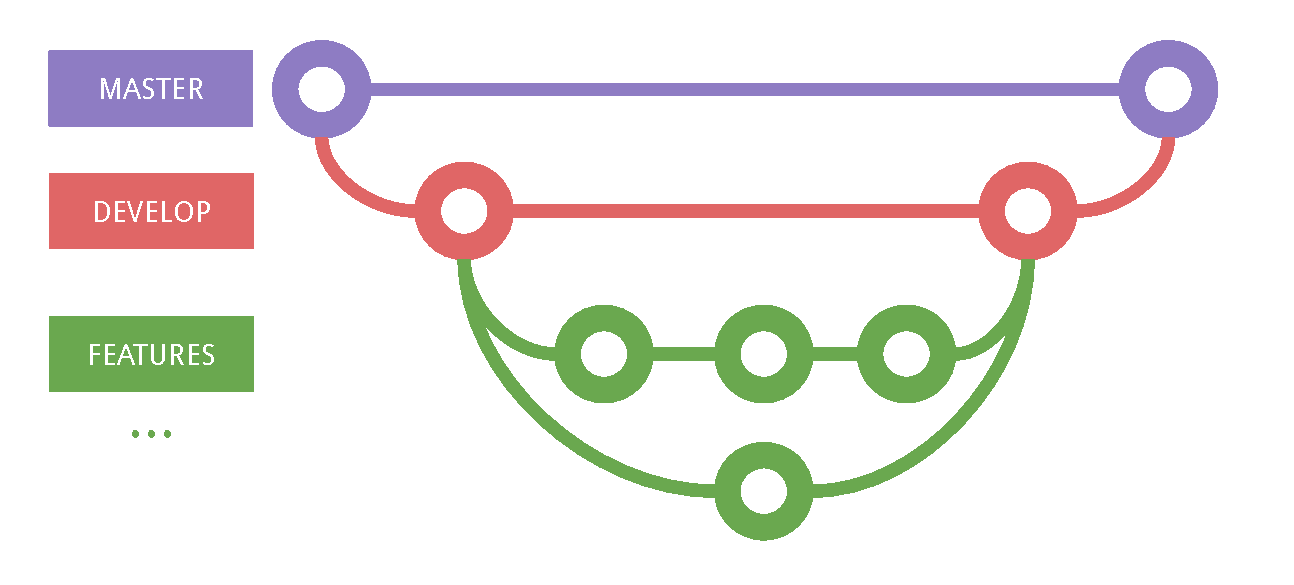
\includegraphics[scale=0.6]{images/gitflow1.pdf}
    \caption{Diagrama del funcionamiento de \textit{GitFlow}}
    \label{fig:gitflow1}
  \end{figure}

Además, nos nutriremos de las buenas prácticas, \textit{librerías} y \textit{repositorios} disponibles en la plataforma,
aprovechando la subida exponencial de la comunidad \textit{Flutter} en este último año, posicionándose
dentro de las tecnologías con más \textit{stars} en el \textit{sitio web}~\cite{gittracker}.

\section{Arquitectura del Sistema}
Una vez definidas las tecnologías que se van a utilizar para el desarrollo de la solución, es importante definir una 
arquitectura que encaje dentro del abanico de requisitos que se desean incluir, además de las funcionalidades que
aportan las tecnologías estudiadas.

Se requiere de una arquitectura de \textit{software}, que no tenga tanta complejidad, ya que no se trata de un
proceso industrial y el desarrollo va a ser realizado por una persona, además de estar bien establecida, ya que
no se quiere entorpecer la escalabilidad del sistema, facilitando, de esta forma, las fases de testeo y mantenimiento.

Para un desarrollo con \textit{Flutter} como \textit{framework} de desarrollo \textit{front-end} y \textit{Firebase}
como infraestructura de servicios \textit{back-end}, se empleará, \textit{la arquitectura por capas}, o 
\textit{Layered Architecture} 
una de las más arquitecturas más conocidas y elegidas en entornos de desarrollo móvil~\cite{7053865}.

\subsection{Arquitectura por capas}
El objetivo de esta arquitectura es la de abstraer lo máximo posible los diferentes bloques o componentes que van a
conformar el sistema. 

Empleando la siguiente arquitectura se pretenderá obtener, a corto y largo plazo,  los siguientes beneficios:

\begin{itemize}
  \item[$\bullet$] Componentes que desempeñan una única funcionalidad bien definida.
  \item[$\bullet$] Mayor escalabilidad, favoreciendo la inclusión de nuevas funcionalidades.
  \item[$\bullet$] Facilidad en la identificación de posibles \textit{bugs} o errores relativos a la
  ejecución del aplicativo.
  \item[$\bullet$] Permite la inclusión de \textit{patrones de diseño} en el sistema.
  \item[$\bullet$] Código más legible y fácil de entender.
\end{itemize}

A partir de esta arquitectura es posible dividir el sistema mediante N bloques, para el aplicativo final se ha optado por una
arquitectura dividida en cuatro capas, como se puede visualizar en la Figura~\ref{fig:architecture1}.

\begin{figure}[H]
  \centering
  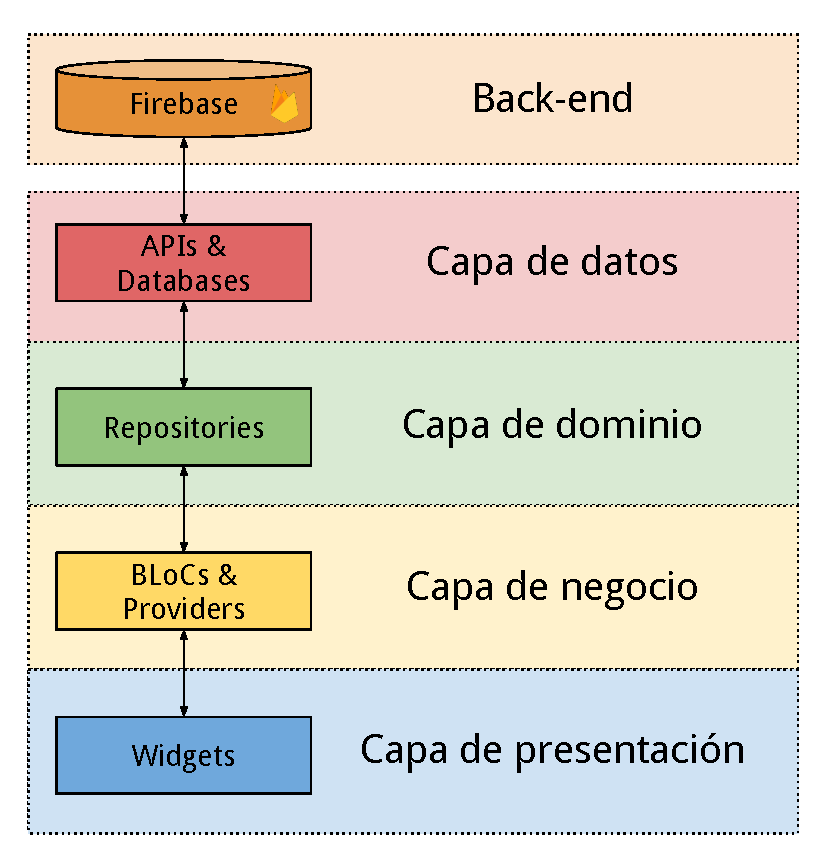
\includegraphics[scale=0.7]{images/architecture.pdf}
  \caption{Diagrama de \textit{Arquitectura basada en cuatro capas}}
  \label{fig:architecture1}
\end{figure}

A continuación, se comentará la funcionalidad de cada una de las capas, en la Tabla~\ref{fig:tablelayers}:

\begin{table}[H]
  \centering
  \caption{Función de las capas de la arquitectura del sistema}
    \begin{tabular}{ | c | c |}
      \hline
      \thead{Capa} & \thead{Funcionalidad} \\
      \hline
      \makecell{Capa de \\ presentación} &  \makecell{Mediante \textit{widgets} se presentarán todas las vistas
      y componentes\\ que contiene el aplicativo.} \\
      \hline
      \makecell{Capa de \\ lógica} &   \makecell{A partir de \textit{manejadores de estados} se controlarán todos los \\ cambios de
      estado presentes en la capa de \textit{presentación}.} \\
      \hline
      \makecell{Capa de \\ dominio} &  \makecell{Las interfaces \textit{repositorio} servirán de esqueleto \\ para las clases relacionadas con
      la capa de \textit{datos}.} \\
      \hline
      \makecell{Capa de \\ datos} &  \makecell{Implementando las interfaces de la capa de \textit{dominio} se
      obtendrán los \\ datos de fuentes externas como nuestro \textit{back-end} de \textit{Firebase}} \\
      \hline
    \end{tabular}
    \label{fig:tablelayers}
\end{table}

Adicionalmente, justo a este modelo de capas se adoptará
la arquitectura \textit{Clean Arquitecture} y la metodología de desarrollo quiado
por pruebas \textit{TDD}, práctica cada vez más vista en proyectos extensos y de gran escalabilidad ~\cite{9071367}.
La combinación de estas dos praxis permitirán modularizar al máximo las funcionalidades del sistema, haciéndolos más
reutilizables y fáciles de monitorizar en las tareas de identificación de errores y rendimiento.

\subsection{Manejador de estados}

Es cierto que \textit{Flutter} permite \textit{manejar} todos los diferentes \textit{estados}, que van surgiendo
en el aplicativo, como por ejemplo: \textit{refrescar de forma dinámica una lista de objetos}; directamente
en la \textit{capa de presentación}, mediante la función \textit{setState()}\cite{flutterState}.

Sin embargo, para nuestra aplicación u otras soluciones de gran envergadura esta tarea puede resultar muy compleja,
además de ser totalmente opuesta a la modulabilidad y reusabilidad que ofrece la arquitectura \textit{Clean Architecture}.
Por ello, se hacen necesarios patrones de diseño que actúen como
\textit{manejadores de estados}, que esté presente en la capa de \textit{lógica} y que se encarguen de:

\begin{itemize}
  \item[$\bullet$] Controlar todos los eventos presentes en el aplicativo 
  para transformarlos en estados y transmitirlos a la capa de \textit{presentación}.
  \item[$\bullet$] Obtener los datos sincronizados transmitidos por la capa de \textit{datos}.
\end{itemize}

Dentro del gran abanico de librerías e implementaciones que ofrece \textit{Flutter} se ha optado por, como se puede 
visualizar en la Figura~\ref{fig:architecture1}, la combinación de los siguientes patrones:

\begin{itemize}
  \item[$\bullet$] \textbf{Patrón BLoC}: empleado para centralizar los cambios de estado, recibiendo \textit{eventos}
   de la capa de \textit{presentación} y transmitir \textit{estados} que cambien de forma dinámica los componentes de
    la misma.
  \item[$\bullet$] \textbf{Provider}: nos permitirá, como su nombre indica, proveer de funcionalidades propias
  de la capa de lógica, como la lógica de los BLoCs a la \textit{capa de presentación}.
\end{itemize}

Esta combinación de patrones se incluirá en el aplicativo mediante el paquete \textit{flutter\_bloc}.
En el capítulo de \textit{Desarrollo de la solución}, se podrá visualizar algunos ejemplos de dicha metodología en
el sistema.
